\documentclass[9pt,english,utf8]{article}

\newcommand{\etal}{\emph{et al.}\@\xspace}

\usepackage{graphicx}
\usepackage{array}
\usepackage{enumerate}
\usepackage{booktabs}
\usepackage{subfigure}
\usepackage{amsmath}
\usepackage{units}
\usepackage{xspace}
\usepackage{caption}
\usepackage{xcolor}
\usepackage{cases}

\graphicspath{{figures/}}

\usepackage{tikz}
\usetikzlibrary{matrix,shapes,arrows,positioning,backgrounds,decorations.pathreplacing,shapes.misc,decorations.text}


\definecolor{a}{HTML}{FFB338}
\definecolor{b}{HTML}{FC6039}
\definecolor{c}{HTML}{FF194D}
\definecolor{d}{HTML}{F73CB5}
\definecolor{e}{HTML}{E63DF4}
\definecolor{f}{HTML}{A54CFF}
\definecolor{g}{HTML}{887FFF}
\definecolor{h}{HTML}{3379FF}
\definecolor{i}{HTML}{42C3E9}
\definecolor{j}{HTML}{43E7C7}
\definecolor{k}{HTML}{44E481}
\definecolor{l}{HTML}{4CE246}
\definecolor{m}{HTML}{43E795}
\definecolor{n}{HTML}{98E246}


\newcommand{\telstart}[2]{
    \pgfmathsetmacro{\x}{#1}
    \pgfmathsetmacro{\y}{#2}
    \fill[color=gray] (\x+0.18, \y+0.16) arc (90:270:0.16 and 0.16) -- (\x+0.18,
    \y+0.16);
}
\newcommand{\telend}[2]{
    \pgfmathsetmacro{\x}{#1}
    \pgfmathsetmacro{\y}{#2}
    \fill[color=gray] (\x, \y+0.16) arc (270:90:-0.16 and -0.16) -- (\x,
    \y+0.16);
}

\newcommand{\gene}[3]{
    \pgfmathsetmacro{\x}{#1}
    \pgfmathsetmacro{\y}{#2}
    \foreach \char [count=\ci] in #3 {
        \fill[draw=none,color=\char] (\x, \y +\ci*0.32 - 0.16) rectangle
        (\x+0.78, \y +\ci*0.32 - 0.48);
        \node[color=black] at (\x+0.39, \y + \ci*0.32 - 0.32) {\textbf{\small\char}};
    }
}
 


\title{Genome Evolution with Horizontal Gene Transfer and Gene Content
Modifications}
\author{Daniel Doerr}
\begin{document}
\maketitle
%\tableofcontents
\section{Introduction}


%Microbial genome evolution
%
%- genome is defined as circular chromosome
%- horizontal gene transfer is a major factor in genome evolution of microbial
%species

This work contributes towards the formulation of a distance measure for the
study of microbial genome evolution. More specifically, it proposes an extension
of the synteny index (SI) distance. 

A \emph{(microbial)} genome $G = g_1\cdot g_2 \cdots g_n$ is defined as a single
circular chromosome constituting a circular sequence of $n$ unoriented genes.
Each gene is represented by its gene family identifier, which is a character
drawn from the alphabet of gene families~$\Sigma$. Within a genome, each gene
family has at most one associated gene.

Subject of this study is the analysis of horizontal gene transfer (HGT), which
plays a major role in microbial genome evolution. At the same time, other
mutations affect microbial genomes, too: (i) point mutations, (ii) genome
rearrangements, (iii) gene content modifications such as (iv) insertions (which
could also be caused by HGT events), deletions, and (v) duplications. 

We aim to study the joint effect of HGT events and gene content modification by
insertions and deletions on the SI distance measure between two genomes $G_x$
and $G_y$, which is defined as follows:

\begin{equation}
    SI(G_x, G_y) := 1 - \left(\frac{1}{2kn} \cdot\sum_{i=1}^{|G_x|} \sum_{j \in
    [i-k, i+k]\setminus \{i\}} \mathcal I_{k}(g_j, g_i, G_y)\right)\,,
\end{equation}
\noindent where

\[\mathcal I_{k}(g, g', G):= \begin{cases} 0 & \textrm{if } g' \not\in G\\
    0 & \textrm{if } g \not\in G[p_G(g')-k,p_G(g')+k] \\
    1 & \textrm{otherwise} \end{cases}
\]

\noindent and $p_H(h)$ denotes the position of gene $h$ in genome $H$. 

\smallskip
An HGT event is modelled as the substitution of an already present gene in the
genome by a (presumably ``better'') homolog. To this end, the old gene is
removed from its current position in the genome, and the new gene is inserted at
a new, arbitrary position:

\begin{center}
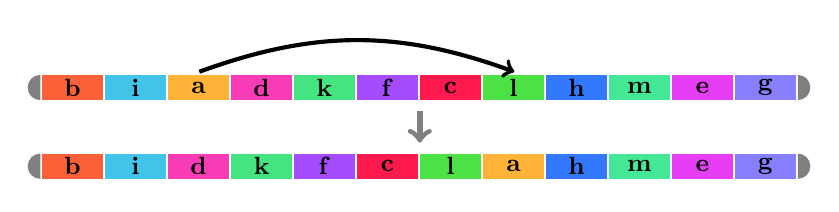
\begin{tikzpicture}
        \telstart{-10.2}{10};
        \gene{-10}{10}{b};
        \gene{-9.2}{10}{i};
        \gene{-8.4}{10}{a};
        \gene{-7.6}{10}{d};
        \gene{-6.8}{10}{k};
        \gene{-6}{10}{f};
        \gene{-5.2}{10}{c};
        \gene{-4.4}{10}{l};
        \gene{-3.6}{10}{h};
        \gene{-2.8}{10}{m};
        \gene{-2}{10}{e};
        \gene{-1.2}{10}{g};
        \telend{-0.4}{10};

        \path[->,bend left=20,color=black,line width=1.5,rounded corners] (-8,
        10.2) edge node {} (-4, 10.2);

        \path[->,color=gray,line width=2] (-5.2, 9.7) edge node {} (-5.2, 9.3);
        
        \telstart{-10.2}{9};
        \gene{-10}{9}{b};
        \gene{-9.2}{9}{i};
        \gene{-8.4}{9}{d};
        \gene{-7.6}{9}{k};
        \gene{-6.8}{9}{f};
        \gene{-6}{9}{c};
        \gene{-5.2}{9}{l};
        \gene{-4.4}{9}{a};
        \gene{-3.6}{9}{h};
        \gene{-2.8}{9}{m};
        \gene{-2}{9}{e};
        \gene{-1.2}{9}{g};
        \telend{-0.4}{9};
\end{tikzpicture}
\end{center}

\section{Gene content modifications}

%- gene content modifications do play an equally important role
%    - new genes are inserted (possibly by means of HGT)
%    - other genes are lost, due to change of ecological niche or other
%    environmental factors
%    - some genes are replaced by analogs
%    
%- a simple model: genome evolution in presence of HGT and gene content evolution
%when genome size is fixed. 

Over a longer evolutionary period of time, the gene content of microbial genomes
is frequently altered by the insertion of new, and the deletion or
pseudogenization of already established genes.  We propose a restricted model
for gene content evolution that does not change the genome size $n$, thus
enabling simplified analysis. In this model, the gene content may only change by
a synchronized deletion and insertion event, subsequently called
``\emph{indel}'', in which an arbitrary gene is substituted by an \emph{indel
gene}, i.e., a gene associated with a novel gene family:

\begin{center}
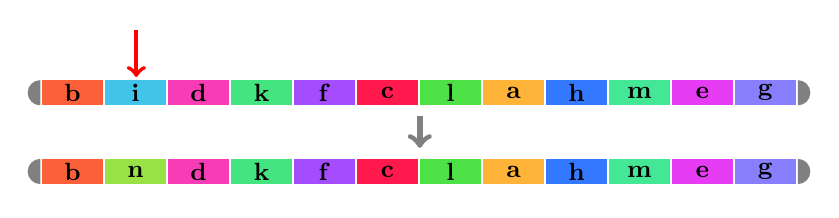
\begin{tikzpicture}
        \path[->,color=red,line width=1.5] (-8.8, 10.8) edge node {} (-8.8, 10.2);
        
        \telstart{-10.2}{10};
        \gene{-10}{10}{b};
        \gene{-9.2}{10}{i};
        \gene{-8.4}{10}{d};
        \gene{-7.6}{10}{k};
        \gene{-6.8}{10}{f};
        \gene{-6}{10}{c};
        \gene{-5.2}{10}{l};
        \gene{-4.4}{10}{a};
        \gene{-3.6}{10}{h};
        \gene{-2.8}{10}{m};
        \gene{-2}{10}{e};
        \gene{-1.2}{10}{g};
        \telend{-0.4}{10};

        \path[->,color=gray,line width=2] (-5.2, 9.7) edge node {} (-5.2, 9.3);

        \telstart{-10.2}{9};
        \gene{-10}{9}{b};
        \gene{-9.2}{9}{n};
        \gene{-8.4}{9}{d};
        \gene{-7.6}{9}{k};
        \gene{-6.8}{9}{f};
        \gene{-6}{9}{c};
        \gene{-5.2}{9}{l};
        \gene{-4.4}{9}{a};
        \gene{-3.6}{9}{h};
        \gene{-2.8}{9}{m};
        \gene{-2}{9}{e};
        \gene{-1.2}{9}{g};
        \telend{-0.4}{9};

\end{tikzpicture}
\end{center}


\noindent Over a long period of time, the gene content of a genome is entirely
replaced by indel genes. At each time step $t$, the genome is subject to
average number of $\mu$ indel events that are uniformly distributed over all
$n$ positions, where $\mu$ is the \emph{indel rate} and corresponds to the rate
of a Poisson process. Then, the probability of a gene not being modified by any
indel event in time interval $[0, t]$ is given by $\rho(t) :=
(1-\frac{\mu}{n})^t$.  Let the average synteny index $\mathit{si}(p, t)$ of a
position $p$ at time $t$ be denoted as follows:

\begin{equation}
    \mathit{si}(p,t) = \begin{cases} 0 & \textrm{if $p$ hosts an indel gene}\\
        2k\rho(t) & \textrm{otherwise,} \end{cases}
\end{equation}

\noindent Consequently, multiplying the two cases by their respective
probabilities of occurrence, we obtain the overall expected synteny index of a
position $E(si(p,t)) = 0 \cdot (1-\rho(t)) + 2k\rho(t)^2$.  This already leads
to a first approximation of the SI distance at time step $t$ between the initial
genome $G_0$ and genome $G_t$:

\begin{equation}
    \widetilde{SI}(G_x, G_y) = 1-\frac{2k\rho(t)^2n}{2kn} = 1-\rho(t)^2
\end{equation}

Consider the increase of the SI distance from time point $t=0$ to $t' :=
t+\varepsilon$. Assume that at time $t'$ a position is hit by an indel event for
the first time, then the distance increases by $\frac{2k}{2kn}$ because of the
loss of the $2k$ neighborhood of the respective gene, and each of its $2k$
neighbors will have a decreased synteny index by one, bringing the total
increase in distance to $\frac{4k}{2kn} = \frac{2}{n}$.  This observation allows
to estimate the SI distance for indel events through a Poisson process with rate
$\frac{2\mu}{n}$. Note that the indel event at time $t'$ for all $n$ positions
occurs with rate $\mu$:

\begin{equation}
    \widehat{SI}(t) = 1-e^{-\frac{2\mu}{n}t}
\end{equation}


%approximation of SI distance 
%- based on assessment of positions that decrease SI
%- based on Poisson distribution

\begin{figure}[tb]
    \centering 
    \subfigure[]{
        \includegraphics[width=0.47\columnwidth]{hgt0:0_indel0:1}
    }
    \subfigure[]{
        \includegraphics[width=0.47\columnwidth]{hgt0:0_indel1:0}
    }
    \caption{SI distance determined empirically by sampling, estimated by
    $\widetilde{SI}$, and $\widehat{SI}$ for a genome of size $n=1000$, $k=20$,
    and (a) indel rate $\mu=0.1$, (b) indel rate $\mu=1.0$. }
    \label{fig:si_distance_hgtonly}
\end{figure}

Figure~\ref{fig:si_distance_hgtonly} visualizes the SI distance estimated by
$\widetilde{SI}$ and $\widehat{SI}$ for a genome of size $n=1000$ and $k=20$ for
$\mu = 0.1$ and $\mu = 1.0$. For reference, the empirically sampled SI distance
is also shown. 

\section{Towards a joint model of HGT and GCM}

In presence of HGT events (that occur at each time step with rate $\gamma$) and
no indel events, the SI distance can be approximated by a Poisson process:

\begin{equation}
    \overline{SI}(t) = \left(1-e^{-\frac{3\gamma}{n}t}\right)
    \left(1-\frac{2k}{n-1}\right)
\end{equation}

This directly leads to a lower bound of the SI distance under HGT and indel
events, as demonstrated in Figure~\ref{fig:si_distance_hgtindel}:

\begin{equation}
    \underline{SI}(t) = \left(1-e^{-\frac{3\gamma+2\mu}{n}t}\right)
    \left(1-\frac{2k\rho(t)}{n-1}\right)
\end{equation}

\begin{figure}[tb]
    \centering 
    \subfigure[]{
        \includegraphics[width=0.47\columnwidth]{hgt1:0_indel0:1}
    }
    \subfigure[]{
        \includegraphics[width=0.47\columnwidth]{hgt1:0_indel1:0}
    }
    \caption{SI distance determined empirically by sampling, estimated by 
    $\underline{SI}$ for a genome of size $n=1000$, $k=20$, HGT rate $\gamma=1$,
    and (a) indel rate $\mu=0.1$, (b) indel rate $\mu=1.0$.  }
    \label{fig:si_distance_hgtindel}
\end{figure}

\end{document}
